\documentclass[border=4pt]{standalone}

\usepackage{amsmath}
\usepackage{tikz}
\usepackage{mathdots}
\usepackage{yhmath}
\usepackage{cancel}
\usepackage{color}
\usepackage{siunitx}
\usepackage{array}
\usepackage{multirow}
\usepackage{amssymb}
\usepackage{gensymb}
\usepackage{tabularx}
\usepackage{booktabs}
\usetikzlibrary{fadings}
\usetikzlibrary{patterns}


\begin{document}
 
     




\tikzset{every picture/.style={line width=0.75pt}} %set default line width to 0.75pt        

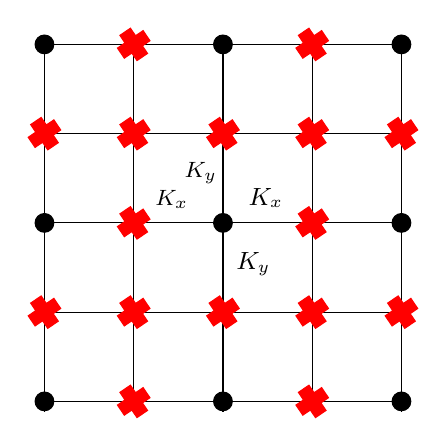
\begin{tikzpicture}[x=0.75pt,y=0.75pt,yscale=-1,xscale=1]
%uncomment if require: \path (0,300); %set diagram left start at 0, and has height of 300

%Shape: Grid [id:dp14968805599998625] 
\draw  [draw opacity=0] (243,90) -- (419.5,90) -- (419.5,267) -- (243,267) -- cycle ; \draw   (243,90) -- (243,267)(286,90) -- (286,267)(329,90) -- (329,267)(372,90) -- (372,267)(415,90) -- (415,267) ; \draw   (243,90) -- (419.5,90)(243,133) -- (419.5,133)(243,176) -- (419.5,176)(243,219) -- (419.5,219)(243,262) -- (419.5,262) ; \draw    ;
%Shape: Circle [id:dp5685771591754973] 
\draw  [color={rgb, 255:red, 0; green, 0; blue, 0 }  ,draw opacity=1 ][fill={rgb, 255:red, 0; green, 0; blue, 0 }  ,fill opacity=1 ] (238.5,90) .. controls (238.5,87.51) and (240.51,85.5) .. (243,85.5) .. controls (245.49,85.5) and (247.5,87.51) .. (247.5,90) .. controls (247.5,92.49) and (245.49,94.5) .. (243,94.5) .. controls (240.51,94.5) and (238.5,92.49) .. (238.5,90) -- cycle ;
%Shape: Circle [id:dp3879309755369156] 
\draw  [color={rgb, 255:red, 0; green, 0; blue, 0 }  ,draw opacity=1 ][fill={rgb, 255:red, 0; green, 0; blue, 0 }  ,fill opacity=1 ] (238.5,176) .. controls (238.5,173.51) and (240.51,171.5) .. (243,171.5) .. controls (245.49,171.5) and (247.5,173.51) .. (247.5,176) .. controls (247.5,178.49) and (245.49,180.5) .. (243,180.5) .. controls (240.51,180.5) and (238.5,178.49) .. (238.5,176) -- cycle ;
%Shape: Circle [id:dp04461290978665855] 
\draw  [color={rgb, 255:red, 0; green, 0; blue, 0 }  ,draw opacity=1 ][fill={rgb, 255:red, 0; green, 0; blue, 0 }  ,fill opacity=1 ] (238.5,262) .. controls (238.5,259.51) and (240.51,257.5) .. (243,257.5) .. controls (245.49,257.5) and (247.5,259.51) .. (247.5,262) .. controls (247.5,264.49) and (245.49,266.5) .. (243,266.5) .. controls (240.51,266.5) and (238.5,264.49) .. (238.5,262) -- cycle ;
%Shape: Circle [id:dp8214471468235309] 
\draw  [color={rgb, 255:red, 0; green, 0; blue, 0 }  ,draw opacity=1 ][fill={rgb, 255:red, 0; green, 0; blue, 0 }  ,fill opacity=1 ] (324.5,262) .. controls (324.5,259.51) and (326.51,257.5) .. (329,257.5) .. controls (331.49,257.5) and (333.5,259.51) .. (333.5,262) .. controls (333.5,264.49) and (331.49,266.5) .. (329,266.5) .. controls (326.51,266.5) and (324.5,264.49) .. (324.5,262) -- cycle ;
%Shape: Circle [id:dp9959417768041545] 
\draw  [color={rgb, 255:red, 0; green, 0; blue, 0 }  ,draw opacity=1 ][fill={rgb, 255:red, 0; green, 0; blue, 0 }  ,fill opacity=1 ] (324.5,176) .. controls (324.5,173.51) and (326.51,171.5) .. (329,171.5) .. controls (331.49,171.5) and (333.5,173.51) .. (333.5,176) .. controls (333.5,178.49) and (331.49,180.5) .. (329,180.5) .. controls (326.51,180.5) and (324.5,178.49) .. (324.5,176) -- cycle ;
%Shape: Circle [id:dp2868907290552285] 
\draw  [color={rgb, 255:red, 0; green, 0; blue, 0 }  ,draw opacity=1 ][fill={rgb, 255:red, 0; green, 0; blue, 0 }  ,fill opacity=1 ] (324.5,90) .. controls (324.5,87.51) and (326.51,85.5) .. (329,85.5) .. controls (331.49,85.5) and (333.5,87.51) .. (333.5,90) .. controls (333.5,92.49) and (331.49,94.5) .. (329,94.5) .. controls (326.51,94.5) and (324.5,92.49) .. (324.5,90) -- cycle ;
%Shape: Cross [id:dp7213219674057381] 
\draw  [color={rgb, 255:red, 255; green, 0; blue, 0 }  ,draw opacity=1 ][fill={rgb, 255:red, 255; green, 0; blue, 0 }  ,fill opacity=1 ] (247.53,126.38) -- (250.82,131.24) -- (247.18,133.71) -- (249.65,137.35) -- (244.58,140.79) -- (242.11,137.15) -- (238.47,139.62) -- (235.18,134.76) -- (238.82,132.29) -- (236.35,128.65) -- (241.42,125.21) -- (243.89,128.85) -- cycle ;
%Shape: Cross [id:dp045925015265155134] 
\draw  [color={rgb, 255:red, 255; green, 0; blue, 0 }  ,draw opacity=1 ][fill={rgb, 255:red, 255; green, 0; blue, 0 }  ,fill opacity=1 ] (419.53,126.38) -- (422.82,131.24) -- (419.18,133.71) -- (421.65,137.35) -- (416.58,140.79) -- (414.11,137.15) -- (410.47,139.62) -- (407.18,134.76) -- (410.82,132.29) -- (408.35,128.65) -- (413.42,125.21) -- (415.89,128.85) -- cycle ;
%Shape: Cross [id:dp8566207093973439] 
\draw  [color={rgb, 255:red, 255; green, 0; blue, 0 }  ,draw opacity=1 ][fill={rgb, 255:red, 255; green, 0; blue, 0 }  ,fill opacity=1 ] (290.53,83.38) -- (293.82,88.24) -- (290.18,90.71) -- (292.65,94.35) -- (287.58,97.79) -- (285.11,94.15) -- (281.47,96.62) -- (278.18,91.76) -- (281.82,89.29) -- (279.35,85.65) -- (284.42,82.21) -- (286.89,85.85) -- cycle ;
%Shape: Cross [id:dp6239487147244225] 
\draw  [color={rgb, 255:red, 255; green, 0; blue, 0 }  ,draw opacity=1 ][fill={rgb, 255:red, 255; green, 0; blue, 0 }  ,fill opacity=1 ] (247.53,212.38) -- (250.82,217.24) -- (247.18,219.71) -- (249.65,223.35) -- (244.58,226.79) -- (242.11,223.15) -- (238.47,225.62) -- (235.18,220.76) -- (238.82,218.29) -- (236.35,214.65) -- (241.42,211.21) -- (243.89,214.85) -- cycle ;
%Shape: Cross [id:dp8354580296018816] 
\draw  [color={rgb, 255:red, 255; green, 0; blue, 0 }  ,draw opacity=1 ][fill={rgb, 255:red, 255; green, 0; blue, 0 }  ,fill opacity=1 ] (290.53,169.38) -- (293.82,174.24) -- (290.18,176.71) -- (292.65,180.35) -- (287.58,183.79) -- (285.11,180.15) -- (281.47,182.62) -- (278.18,177.76) -- (281.82,175.29) -- (279.35,171.65) -- (284.42,168.21) -- (286.89,171.85) -- cycle ;
%Shape: Cross [id:dp8854453213367393] 
\draw  [color={rgb, 255:red, 255; green, 0; blue, 0 }  ,draw opacity=1 ][fill={rgb, 255:red, 255; green, 0; blue, 0 }  ,fill opacity=1 ] (333.53,126.38) -- (336.82,131.24) -- (333.18,133.71) -- (335.65,137.35) -- (330.58,140.79) -- (328.11,137.15) -- (324.47,139.62) -- (321.18,134.76) -- (324.82,132.29) -- (322.35,128.65) -- (327.42,125.21) -- (329.89,128.85) -- cycle ;
%Shape: Cross [id:dp23014117299749937] 
\draw  [color={rgb, 255:red, 255; green, 0; blue, 0 }  ,draw opacity=1 ][fill={rgb, 255:red, 255; green, 0; blue, 0 }  ,fill opacity=1 ] (333.53,212.38) -- (336.82,217.24) -- (333.18,219.71) -- (335.65,223.35) -- (330.58,226.79) -- (328.11,223.15) -- (324.47,225.62) -- (321.18,220.76) -- (324.82,218.29) -- (322.35,214.65) -- (327.42,211.21) -- (329.89,214.85) -- cycle ;
%Shape: Cross [id:dp007744491742833981] 
\draw  [color={rgb, 255:red, 255; green, 0; blue, 0 }  ,draw opacity=1 ][fill={rgb, 255:red, 255; green, 0; blue, 0 }  ,fill opacity=1 ] (419.53,212.38) -- (422.82,217.24) -- (419.18,219.71) -- (421.65,223.35) -- (416.58,226.79) -- (414.11,223.15) -- (410.47,225.62) -- (407.18,220.76) -- (410.82,218.29) -- (408.35,214.65) -- (413.42,211.21) -- (415.89,214.85) -- cycle ;
%Shape: Cross [id:dp05057141321991909] 
\draw  [color={rgb, 255:red, 255; green, 0; blue, 0 }  ,draw opacity=1 ][fill={rgb, 255:red, 255; green, 0; blue, 0 }  ,fill opacity=1 ] (290.53,126.38) -- (293.82,131.24) -- (290.18,133.71) -- (292.65,137.35) -- (287.58,140.79) -- (285.11,137.15) -- (281.47,139.62) -- (278.18,134.76) -- (281.82,132.29) -- (279.35,128.65) -- (284.42,125.21) -- (286.89,128.85) -- cycle ;
%Shape: Cross [id:dp08720775969693806] 
\draw  [color={rgb, 255:red, 255; green, 0; blue, 0 }  ,draw opacity=1 ][fill={rgb, 255:red, 255; green, 0; blue, 0 }  ,fill opacity=1 ] (290.53,255.38) -- (293.82,260.24) -- (290.18,262.71) -- (292.65,266.35) -- (287.58,269.79) -- (285.11,266.15) -- (281.47,268.62) -- (278.18,263.76) -- (281.82,261.29) -- (279.35,257.65) -- (284.42,254.21) -- (286.89,257.85) -- cycle ;
%Shape: Cross [id:dp4819369844802004] 
\draw  [color={rgb, 255:red, 255; green, 0; blue, 0 }  ,draw opacity=1 ][fill={rgb, 255:red, 255; green, 0; blue, 0 }  ,fill opacity=1 ] (290.53,212.38) -- (293.82,217.24) -- (290.18,219.71) -- (292.65,223.35) -- (287.58,226.79) -- (285.11,223.15) -- (281.47,225.62) -- (278.18,220.76) -- (281.82,218.29) -- (279.35,214.65) -- (284.42,211.21) -- (286.89,214.85) -- cycle ;
%Shape: Cross [id:dp004713105281045404] 
\draw  [color={rgb, 255:red, 255; green, 0; blue, 0 }  ,draw opacity=1 ][fill={rgb, 255:red, 255; green, 0; blue, 0 }  ,fill opacity=1 ] (376.53,212.38) -- (379.82,217.24) -- (376.18,219.71) -- (378.65,223.35) -- (373.58,226.79) -- (371.11,223.15) -- (367.47,225.62) -- (364.18,220.76) -- (367.82,218.29) -- (365.35,214.65) -- (370.42,211.21) -- (372.89,214.85) -- cycle ;
%Shape: Cross [id:dp10093717545960956] 
\draw  [color={rgb, 255:red, 255; green, 0; blue, 0 }  ,draw opacity=1 ][fill={rgb, 255:red, 255; green, 0; blue, 0 }  ,fill opacity=1 ] (376.53,169.38) -- (379.82,174.24) -- (376.18,176.71) -- (378.65,180.35) -- (373.58,183.79) -- (371.11,180.15) -- (367.47,182.62) -- (364.18,177.76) -- (367.82,175.29) -- (365.35,171.65) -- (370.42,168.21) -- (372.89,171.85) -- cycle ;
%Shape: Cross [id:dp2597413862979294] 
\draw  [color={rgb, 255:red, 255; green, 0; blue, 0 }  ,draw opacity=1 ][fill={rgb, 255:red, 255; green, 0; blue, 0 }  ,fill opacity=1 ] (376.53,126.38) -- (379.82,131.24) -- (376.18,133.71) -- (378.65,137.35) -- (373.58,140.79) -- (371.11,137.15) -- (367.47,139.62) -- (364.18,134.76) -- (367.82,132.29) -- (365.35,128.65) -- (370.42,125.21) -- (372.89,128.85) -- cycle ;
%Shape: Cross [id:dp5866249907711081] 
\draw  [color={rgb, 255:red, 255; green, 0; blue, 0 }  ,draw opacity=1 ][fill={rgb, 255:red, 255; green, 0; blue, 0 }  ,fill opacity=1 ] (376.53,83.38) -- (379.82,88.24) -- (376.18,90.71) -- (378.65,94.35) -- (373.58,97.79) -- (371.11,94.15) -- (367.47,96.62) -- (364.18,91.76) -- (367.82,89.29) -- (365.35,85.65) -- (370.42,82.21) -- (372.89,85.85) -- cycle ;
%Shape: Cross [id:dp07887008563662223] 
\draw  [color={rgb, 255:red, 255; green, 0; blue, 0 }  ,draw opacity=1 ][fill={rgb, 255:red, 255; green, 0; blue, 0 }  ,fill opacity=1 ] (376.53,255.38) -- (379.82,260.24) -- (376.18,262.71) -- (378.65,266.35) -- (373.58,269.79) -- (371.11,266.15) -- (367.47,268.62) -- (364.18,263.76) -- (367.82,261.29) -- (365.35,257.65) -- (370.42,254.21) -- (372.89,257.85) -- cycle ;
%Shape: Circle [id:dp769670819937206] 
\draw  [color={rgb, 255:red, 0; green, 0; blue, 0 }  ,draw opacity=1 ][fill={rgb, 255:red, 0; green, 0; blue, 0 }  ,fill opacity=1 ] (410.5,90) .. controls (410.5,87.51) and (412.51,85.5) .. (415,85.5) .. controls (417.49,85.5) and (419.5,87.51) .. (419.5,90) .. controls (419.5,92.49) and (417.49,94.5) .. (415,94.5) .. controls (412.51,94.5) and (410.5,92.49) .. (410.5,90) -- cycle ;
%Shape: Circle [id:dp8092618925934953] 
\draw  [color={rgb, 255:red, 0; green, 0; blue, 0 }  ,draw opacity=1 ][fill={rgb, 255:red, 0; green, 0; blue, 0 }  ,fill opacity=1 ] (410.5,176) .. controls (410.5,173.51) and (412.51,171.5) .. (415,171.5) .. controls (417.49,171.5) and (419.5,173.51) .. (419.5,176) .. controls (419.5,178.49) and (417.49,180.5) .. (415,180.5) .. controls (412.51,180.5) and (410.5,178.49) .. (410.5,176) -- cycle ;
%Shape: Circle [id:dp7356173827687185] 
\draw  [color={rgb, 255:red, 0; green, 0; blue, 0 }  ,draw opacity=1 ][fill={rgb, 255:red, 0; green, 0; blue, 0 }  ,fill opacity=1 ] (410.5,262) .. controls (410.5,259.51) and (412.51,257.5) .. (415,257.5) .. controls (417.49,257.5) and (419.5,259.51) .. (419.5,262) .. controls (419.5,264.49) and (417.49,266.5) .. (415,266.5) .. controls (412.51,266.5) and (410.5,264.49) .. (410.5,262) -- cycle ;

% Text Node
\draw (304.33,164.67) node  [font=\footnotesize]  {$K_{x}$};
% Text Node
\draw (349.67,164) node  [font=\small]  {$K_{x}$};
% Text Node
\draw (318.33,152) node  [font=\footnotesize]  {$K_{y}$};
% Text Node
\draw (343.67,196) node  [font=\small]  {$K_{y}$};


\end{tikzpicture}

\end{document}
